\section{Bilder}

\ref{fig:zeitreihe-komponenten} wurde mit dem Python Skript \verb|skripte/plot_zeitreihe_komponenten.py| erstellt.

\begin{figure}[h]
  \centering
  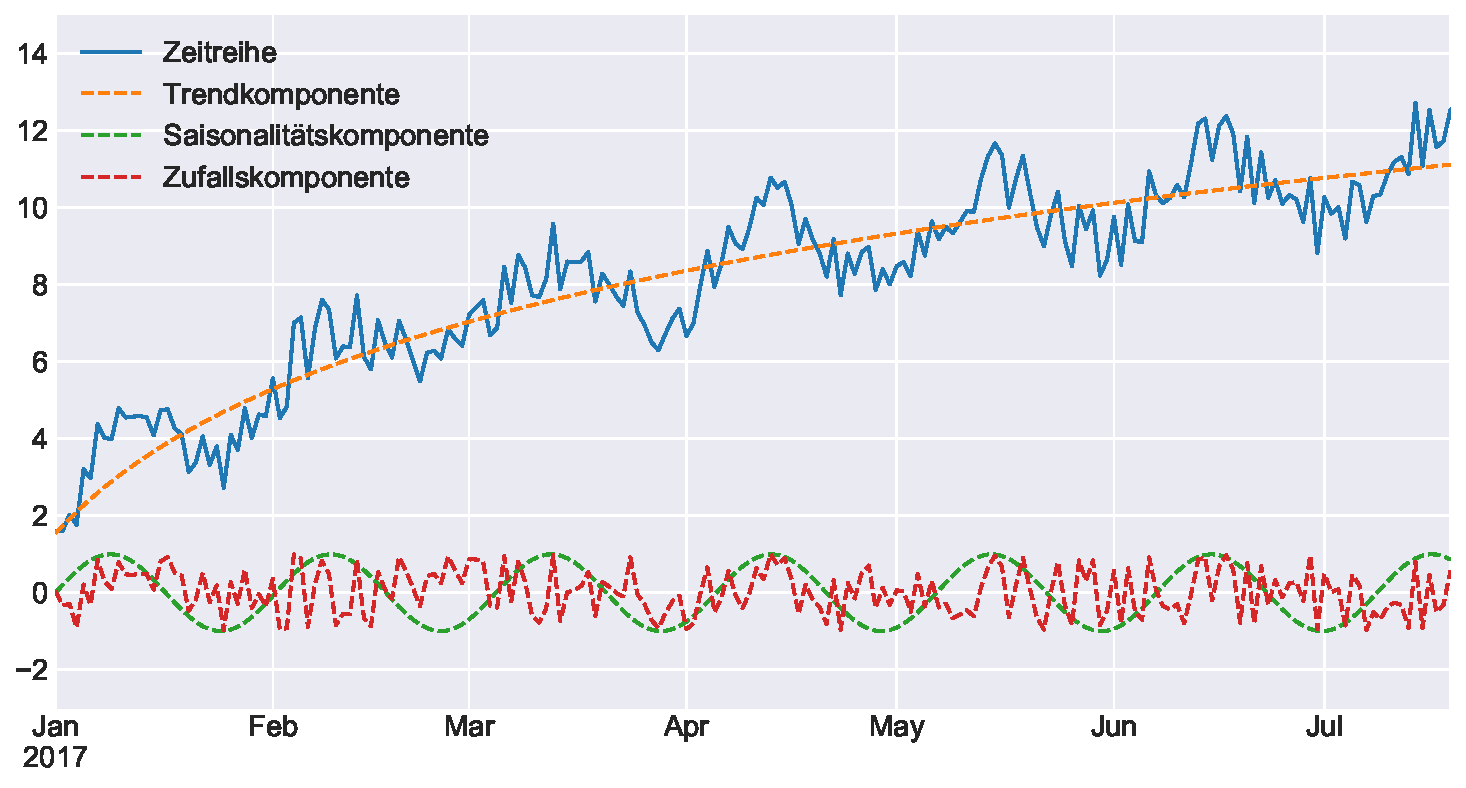
\includegraphics[width=\textwidth]{bilder/02-hauptteil/zeitreihe-komponenten.pdf}
  \caption[Aufteilung einer Zeitreihe in mehrere Komponenten]{Aufteilung einer Zeitreihe in mehrere Komponenten. Bild entnommen aus \citet{Masterthesis.2017}.}
  \label{fig:zeitreihe-komponenten}
\end{figure}

Und hier nochmal zwei Abbildungen (\ref{fig:zeitreihe-komponenten2}, \ref{fig:zeitreihe-komponenten3}) in zwei Spalten mit jeweils eigenen Abbildungsbeschriftungen.

\begin{figure}[ht]
  \parbox{.47\textwidth}{
    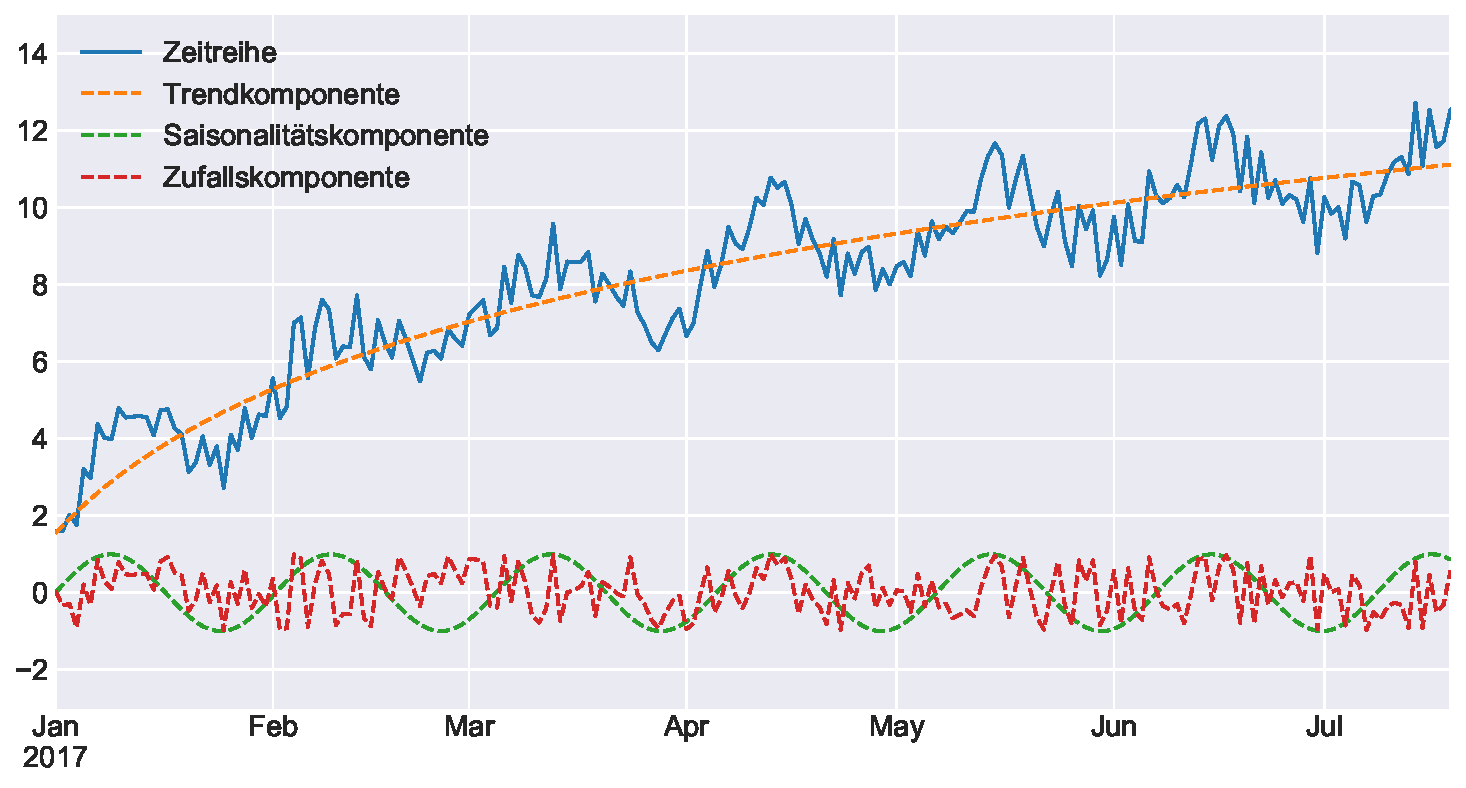
\includegraphics[width=0.47\textwidth]{bilder/02-hauptteil/zeitreihe-komponenten.pdf}
    \caption[Aufteilung einer Zeitreihe in mehrere Komponenten]{Aufteilung einer Zeitreihe in mehrere Komponenten. Bild entnommen aus \citet{Masterthesis.2017}.}
    \label{fig:zeitreihe-komponenten2}
  }
  \hfill
  \parbox{.47\textwidth}{
    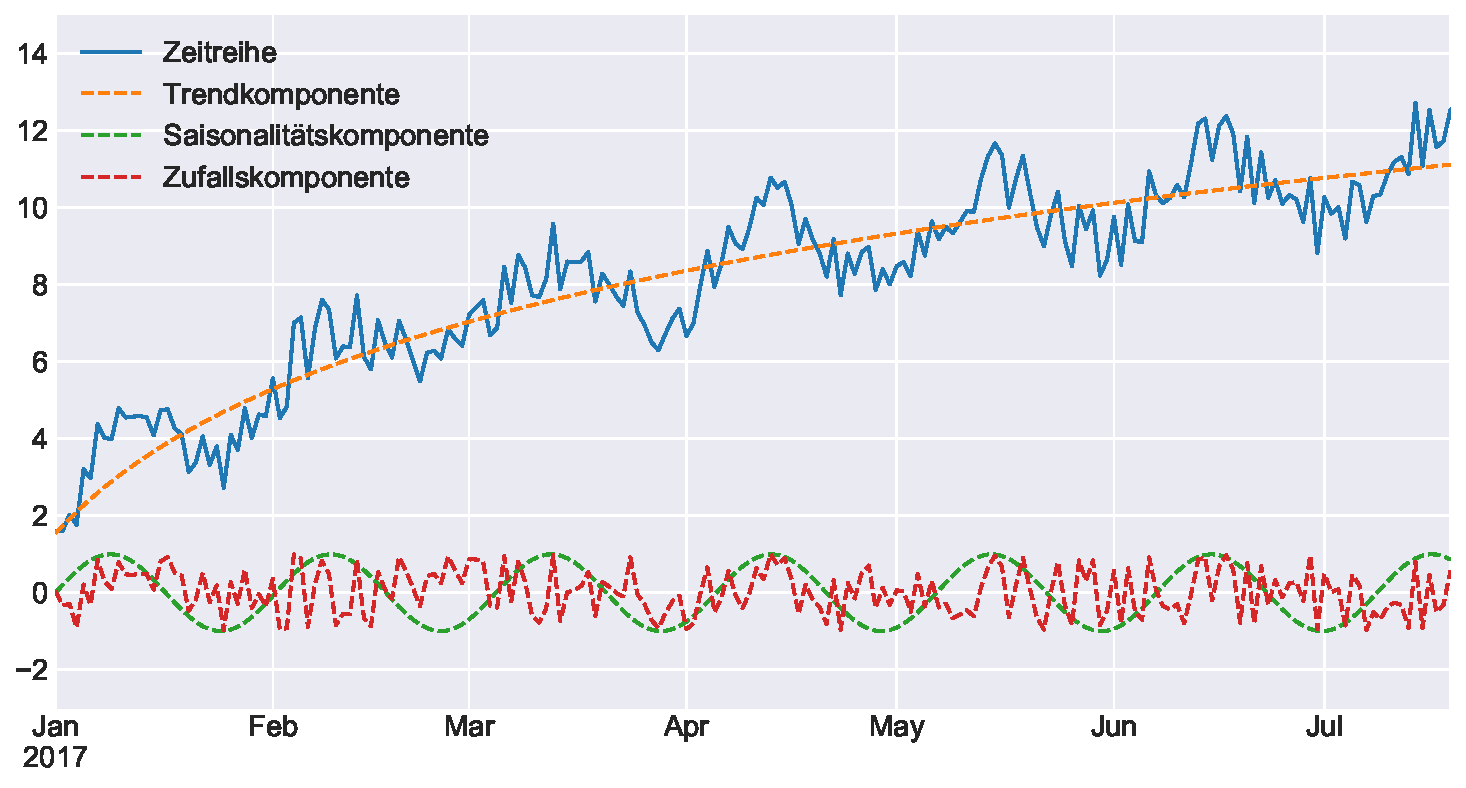
\includegraphics[width=0.47\textwidth]{bilder/02-hauptteil/zeitreihe-komponenten.pdf}
    \caption[Aufteilung einer Zeitreihe in mehrere Komponenten]{Aufteilung einer Zeitreihe in mehrere Komponenten. Bild entnommen aus \citet{Masterthesis.2017}.}
    \label{fig:zeitreihe-komponenten3}
  }
\end{figure}
